\chapter{Versuchsauswertung}\label{s:auswertung}

\section{Referenzmessungen und Ergebnisse bei konstanter Aktuation}
\label{sec:ErgebnisseKonstanteAktuation}

\section{Periodische Aktuation}
\subsection{Ausrichtungsmessungen (FT)}
\label{subs:Vorueberlegungen}

Um die periodische Aktuation zu erm"oglichen, werden die glatten, zylindrischen Wellen aus Aluminium gegen die in \abschn{s:rotierendeWalzen} beschriebenen Wellen getauscht.

Nach dem Einbau wurde erneut die Druckverteilung auf der Oberfl"ache des Modells vorgenommen, um eine optimale Postion des Modells ohne Anstellwinkel zu gew"ahrleisten. Die Ergebnisse sind in \abb{fig:Oberflaechendruckverteilung 50}
zu sehen.

	\begin{figure}[h]
	\centering
	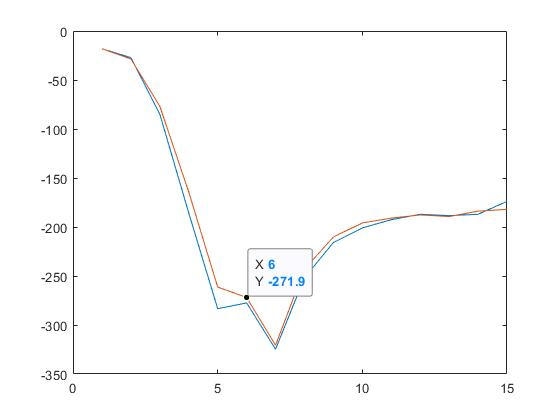
\includegraphics[width=0.8\textwidth]{Oberflaechendruckverteilung50.jpg}
	\caption{Oberfl"achendr"ucke beim eingebauten Modell mit Teflonwalzen}
	\label{fig:Oberflaechendruckverteilung 50}
	\end{figure}

Die D"rucke an der Ober- und Unterseite sind hier wieder gespiegelt und "ubereinandergelegt dargestellt. Der erste Messpunkt entspricht dabei der Druckmessbohrung, die mittig an der Vorderseite eingebracht ist.

Die gr"o\ss{}te Abweichung erf"ahrt der Druck an Ober- und Unterseite genau dort, wo auf beiden Seiten das Zackenband angebracht wurde. Der lokale, jeweilige Abstand der Druckmessbohrung zum Zackenband ist allerdings oben und unten nicht komplett einheitlich. Dies hat zur Folge, dass das Str"omungsverhalten an diesen Orten voneinander abweicht, wodurch die Differenz zu erkl"aren ist.
Da die Druckmessbohrungen im Folgenden keine gro\ss{}e Relevanz haben, ist diese Ungleichm"a\ss{}igkeit kein Problem.

Weiterhin ergibt sich allerdings im Unterschied zu den Messungen der Oberfl"achendr"ucke in \abschn{sec:ErgebnisseKonstanteAktuation} eine leichte Druckerh"ohung an der Oberseite zur letzten Druckmessbohrung hin.
Auch in der Arbeit von \emph{Bilges} \,\cite{Bilges.2018}, die das gleiche Modell als Gegenstand der Untersuchung hatte,ist eine "ahnliche Entwicklung bei niedrigeren Reynoldszahlen als 50.000 zu sehen gewesen.
Die beschriebene Tendenz war aber bei h"oheren Reynoldszahlen wieder kaum wahrnehmbar.


Diese Erscheinung lie\ss{} sich auch nach "Uberpr"ufung der Schl"auche und Bohrungen auf Verunreinigungen bzw. Verstopfungen und mehreren Nachjustierungen der Modellpostion nicht beseitigen.

Auch der m"ogliche Einfluss der oberen und unteren Walze auf diese Werte durch etwaiges leichtes Aufbiegen der Spalte in variierenden Walzenstellungen wurde ohne positive Ver"anderung getestet.

Das Auseinanderstreben der Messwerte ist somit wahrscheinlich auf die in \cite{Bilges.2018} angef"uhrten einseitigen Fertigungstoleranzen und Unebenheiten zur"uckzuf"uhren, welche je nach individueller Einstellung der Spalte bei den verschiedenen Walzenpaaren unterschiedlich stark zum Vorschein kommen.

Da an den anderen Messpunkten Ober- und Unterseite sehr "ahnliche Werte liefern, kann davon ausgegangen werden, dass das Modell symmetrisch in der Anstr"omung platziert ist.


Die eigentlichen Messreihen gestalteten sich bei dieser Konfiguration aus verschiedenen Gr"unden als schwieriger und aufw"andiger als bei der Konfiguration aus \abschn{sec:ErgebnisseKonstanteAktuation}.

%Damit lokale
%
%Phasenungleicheit bei der Wellenrotation.:
%
%Da nicht ausgeschlossen werden kann, dass die beiden Walzen beim Hochfahren der Drehzahl asynchron laufen und sich eine phasenversetzte Aktuation an Ober- und Unterseite ergibt, wurden zu jeder Kombination der Messparameter mehrere Messungen durchgef"uhrt.
%
%Eine 
\section{Effizienzbetrachtung}
